\documentclass{homework}
\newcommand{\R}{\textbf{R}}
\newcommand{\dee}{\;\text{d}}
\newcommand{\eps}{\varepsilon}
\newcommand{\pl}[2]{\frac{\partial #1}{\partial #2}}
\newcommand{\dl}[2]{\frac{\text{d} #1}{\text{d} #2}}
\newcommand{\sgn}{\text{sgn}}
\newcommand{\bigoh}{\mathcal{O}}
\usepackage{enumitem}

\newcommand{\hwclass}{Math 6108}
\newcommand{\hwname}{Jacob Hauck}
\newcommand{\hwtype}{Homework}


\newcommand{\hwnum}{2}
\renewcommand{\questiontype}{Problem}

\begin{document}
	\maketitle
	
	\question 
	
	Consider the IVP
	\begin{equation}
		\label{eq:ivp}
		y' = f(t,y), \qquad y(0) = a.
	\end{equation}
	Let $k > 0$ be the time step for a numerical scheme to approximate $y'$. Assume that $f$ is $L$-Lipschitz in $y$ for all $t$.
	
	\begin{enumerate}
		\item Consider the scheme
		\begin{equation}
			y^{n+1} = y^n + k f\big(t_{n+1}, y^{n+1}\big), \quad n = 0, 1, 2, \dots, \qquad y^0 = a.
		\end{equation}
		Suppose that $y(t_n) = y^n$. Using the Taylor expansion of $y$ about $t_{n+1}$,
		\begin{equation*}
			y(t_n) = y(t_{n+1}) - ky'(t_{n+1}) + \tau(k),
		\end{equation*}
		where the remainder $\tau(k) = \bigoh(k^2)$ as $k\to 0$.
		Using the assumption that $y(t_n) = y^n$ and the definition of the scheme, we have
		\begin{align*}
			y(t_{n+1}) &= y(t_n) + ky'(t_{n+1}) + \tau(k) \\
			&= y^n + kf\big(t_{n+1}, y^{n+1}\big) + k\left[f(t_{n+1},y(t_{n+1})) - f\big(t_{n+1},y^{n+1}\big)\right] + \tau(k) \\
			&= y^{n+1} + k\left[f(t_{n+1},y(t_{n+1})) - f\big(t_{n+1},y^{n+1}\big)\right] + \tau(k).
		\end{align*}
		Thus,
		\begin{equation*}
			\text{LTE} = \big|y(t_{n+1}) - y^{n+1}\big| = \left|k\big[f(t_{n+1},y(t_{n+1})) - f\big(t_{n+1},y^{n+1}\big)\big] + \tau(k)\right|.
		\end{equation*}
		We can easily show that $\text{LTE} \to 0$ as $k\to 0$, that is, that the scheme is consistent.
		
		By the Lipschitz condition on $f$,
		\begin{align*}
			\text{LTE} = \big|y(t_{n+1})-y^{n+1}\big| &\le k\left|f(t_{n+1},y(t_{n+1})) - f\big(t_{n+1},y^{n+1}\big)\right| + |\tau(k)|\\
			&\le kL\big|y(t_{n+1})-y^{n+1}\big| + |\tau(k)|.
		\end{align*}
		For all $k < \frac{1}{L}$, we have $1-kL > 0$, so
		\begin{equation*}
			\text{LTE} \le \frac{|\tau(k)|}{1-kL}, \qquad k < \frac{1}{L}.
		\end{equation*}
		This implies that
		\begin{equation*}
			0 \le \lim_{k\to 0}\text{LTE} \le \lim_{k\to0}\frac{|\tau(k)|}{1-kL} = 0
		\end{equation*}
		because $\tau(k) \to 0$ as $k \to 0$, and $1-kL \to 1$ as $k\to 0$. That is, $\text{LTE} \to 0$ as $k\to0$, and the scheme is consistent.
		
		\item Consider the scheme
		\begin{equation}
			y^{n+1} = y^{n-1} + 2kf(t_n, y_n),\quad n = 0, 1, 2, \dots, \qquad y^0 = a.
		\end{equation}
		Suppose that $y(t_{n-1}) = y^{n-1}$, and $y(t_n) = y^n$. Using the Taylor expansion of $y$ about $t_n$ to the left and to the right, we have
		\begin{align*}
			y(t_{n+1}) &= y(t_n) + ky'(t_n) + \tau_1(k) \\
			y(t_{n-1}) &= y(t_n) - ky'(t_n) + \tau_2(k),
		\end{align*}
		where the remainders $\tau_1(k)$ and $\tau_2(k)$ satisfy $\tau_1(k) = \bigoh(k^2)$ and $\tau_2(k) = \bigoh(k^2)$ as $k \to 0$.
		
		By the ODE and the assumptions that $y(t_{n-1}) = y^{n-1}$ and $y(t_n) = y^n$, this implies that
		\begin{align*}
			y(t_{n+1}) - y^{n-1} &= y(t_{n+1}) -y(t_{n-1}) \\
			&= 2ky'(t_n) +\tau_1(k) - \tau_2(k) \\
			&= 2kf(t_n, y(t_n)) + \tau_1(k) - \tau_2(k) \\
			&= 2kf(t_n, y^n) + \tau_1(k) - \tau_2(k).
		\end{align*}
		Therefore, the $\text{LTE}$ is given by
		\begin{equation*}
			\text{LTE} = \big|y^{n+1} - y(t_{n+1})\big| = |\tau_1(k) - \tau_2(k)|.
		\end{equation*}
		Since both $\tau_1(k) \to 0$ and $\tau_2(k) \to 0$ as $k\to 0$, it follows that $\text{LTE}\to 0$ as $k\to0$. That is, the scheme is consistent.
		
		\item Let $\theta \in [0,1]$, and consider the scheme
		\begin{equation}
			y^{n+1} = y^n + kf\left(t^n + (1-\theta)k, \theta y^n + (1-\theta)y^{n+1}\right),\quad n = 0, 1, 2, \dots, \qquad y^0 = a.
		\end{equation}
		
		Suppose that $y(t_n) = y^n$. Using the Taylor expansion of $y$ about $t_n + (1-\theta)k$, we have
		\begin{equation}
			\label{eq:yt_n}
			y(t_n) = y(t_n + (1-\theta)k) - (1-\theta)ky'(t_n + (1-\theta)k) + \tau_1(k),
		\end{equation}
		where $\tau_1(k) = \bigoh(k^2)$ as $k \to 0$ (because $\theta \in [0,1]$). Similarly,
		\begin{equation}
			\label{eq:yt_np1}
			y(t_{n+1}) = y(t_n + (1-\theta)k) + \theta ky'(t_n + (1-\theta)k) + \tau_2(k),
		\end{equation}
		where $\tau_2(k) = \bigoh(k^2)$ as $k \to 0$. Therefore,
		\begin{align*}
			y(t_{n+1}) &= y(t_n) + (1-\theta)ky'(t_n+(1-\theta)k) -\tau_1(k) + \theta ky'(t_n+(1-\theta)k) + \tau_2(k) \\
			&= y(t_n) + ky'(t_n + (1-\theta)k) - \tau_1(k) + \tau_2(k) \\
			&= y^n + kf(t_n + (1-\theta)k, y(t_n+(1-\theta)k)) -\tau_1(k) + \tau_2(k).
		\end{align*}
		Then the local truncation error is given by
		\begin{align*}
			\text{LTE} &= \left|y(t_{n+1}) - y^{n+1}\right| \\
			&= \left|k\big[f(t_n+(1-\theta)k, y(t_n+(1-\theta)k)) - f\big(t_n+(1-\theta)k, \theta y^n + (1-\theta)y^{n+1}\big)\big] -\tau_1(k) + \tau_2(k)\right|.
		\end{align*}
		By the Lipschitz property of $f$, we have
		\begin{equation*}
			\text{LTE} \le kL\left|y(t_n + (1-\theta)k) - \theta y^n - (1-\theta)y^{n+1}\right| + |\tau_2(k) - \tau_1(k)|.
		\end{equation*}
		Multiplying (\ref{eq:yt_n}) by $\theta$ and (\ref{eq:yt_np1}) by $1-\theta$ and adding the results, we see that
		\begin{equation*}
			y(t_n+(1-\theta)k) = \theta y(t_n) + (1-\theta)y(t_{n+1}) + \theta\tau_1(k) + (1-\theta)\tau_2(k).
		\end{equation*}
		Since $y(t_n) = y^n$ by hypothesis, we have
		\begin{equation*}
			\text{LTE} \le kL(1-\theta)\left|y(t_{n+1}) - y^{n+1}\right| + \tau(k),
		\end{equation*}
		where $\tau(k) = \left|\theta \tau_1(k) + (1-\theta)\tau_2(k)\right| + \left|\tau_2(k) - \tau_1(k)\right|$. If $\theta = 1$, then clearly $\text{LTE} \to 0$ as $k \to 0$. Otherwise, for all $k < \frac{1}{L(1-\theta)}$, we have $1 - kL(1-\theta) > 0$, so
		\begin{equation*}
			\text{LTE} \le \frac{\tau(k)}{1-kL(1-\theta)}, \qquad k < \frac{1}{1 - kL(1-\theta)}.
		\end{equation*}
		Hence,
		\begin{equation*}
			0 \le \lim_{k\to 0}\text{LTE} \le \lim_{k\to 0}\frac{\tau(k)}{1-kL(1-\theta)} = 0
		\end{equation*}
		because $\tau(k) \to 0$ and $1-kL(1-\theta) \to 1$ as $k \to 0$. Therefore, $\text{LTE} \to 0$ as $k \to 0$ for any $\theta \in [0,1]$, and the scheme is consistent.
	\end{enumerate}
	
	\question
	
	Consider the IVP
	\begin{equation}
		\label{eq:p2_ivp}
		y'(t) = \frac{1}{1+t^2} - 2y^2, \quad t >0; \qquad y(0) = 0.
	\end{equation}
	We will discretize this problem by using scheme 3 from Problem 1 on the interval $[0,2]$. Note that this scheme is implicit, so the implementation of it is a straightforward generalization of the implementation of the backward Euler method. The main difference is the construction of the implicit function $f_n$ such that $f_n\left(y^{n+1}\right)=0$. 
	
	In the case of IVP (\ref{eq:p2_ivp}), we have
	\begin{equation*}
		f(t,y) = \frac{1}{1+t^2} - 2y^2, \qquad a = 0.
	\end{equation*}
	Rewriting the equation for $y^{n+1}$ in the definition of the scheme, we get
	\begin{equation*}
		y^{n+1} - y^n - kf\left(t_n + (1-\theta)k, \theta y^n + (1-\theta)y^{n+1}\right) = 0, \quad n = 0, 1, \dots,
	\end{equation*}
	so we can find $y^{n+1}$ by finding a root of
	\begin{equation*}
		f_n(x) = x - y^n - k\left[\frac{1}{1+(t_n + (1-\theta)k)^2} - 2(\theta y^n + (1-\theta)x)^2\right].
	\end{equation*}
	We find this root numerically using Newton's method, which means we need to calculate $f_n'$:
	\begin{equation*}
		f_n'(x) = 1 + 4k(1-\theta)(\theta y^n + (1-\theta)x).
	\end{equation*}
	If $\{x_j\}$ is the sequence of Newton's method approximations of the root, then we use the stopping criterion $|x_j - x_{j-1}| < 10^{-8}$, where $x_j$ is the returned approximation.
	
	The code for running the scheme with given values of the parameters $k$ and $\theta$ is given in \lstinline{problem2.m}. Note that this refers to \lstinline{newton.m}, which is the same implementation of Newton's method from the previous homework.
	
	\lstinputlisting[language=MATLAB, numbers=left, frame=single, basicstyle=\small\ttfamily, showstringspaces=false, caption={\lstinline{problem2.m}, which solves IVP (\ref{eq:p2_ivp}) using scheme 3}, label={lst:problem2}]{problem2.m}
	
	\begin{enumerate}
		\item Consider the case $\theta = 1$.
		\begin{enumerate}[label={(\alph*)}]
			\item To create a plot of the numerical solution on the interval $[0,2]$, we need to choose a small enough $k$ value. We choose $k = \frac{1}{2048}$ for consistency with the value used in the reference solution in subsequent parts. The resulting plot is given in Figure \ref{fig:p2_part1}. Additionally, the numerical value of $y(2)$ is given in \lstinline{problem2_output.txt} as 0.400024. These results can be obtained by running the following excerpt from \lstinline{problem2_calculations.m}.
			
			\lstinputlisting[language=MATLAB, numbers=left, frame=single, basicstyle=\small\ttfamily, showstringspaces=false, caption={Problem 2.1 (a)}, label={lst:p2:1:a}, firstline=5, lastline=20]{problem2_calculations.m}
			
			\begin{figure}[h]
				\centering
				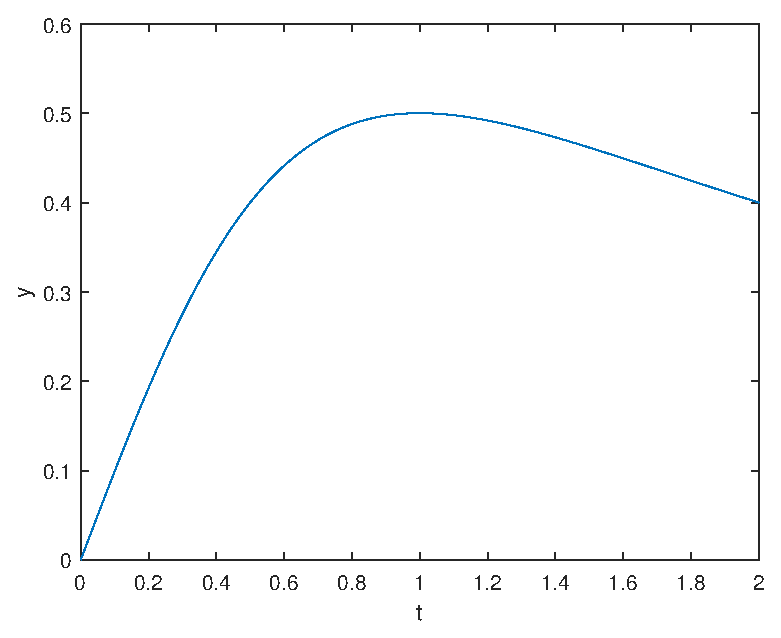
\includegraphics{p2_1_plot.eps}
				\caption{The numerical solution of (\ref{eq:p2_ivp}) on $[0,2]$ with $k = \frac{1}{2048}$ and $\theta = 1$}
				\label{fig:p2_part1}
			\end{figure}
			
			\item The following excerpt (Listing \ref{lst:p2:1:b}) from \lstinline{problem2_calculations.m} computes a reference solution with $k = \frac{1}{2048}$ then calculates the errors at $t=2$ between the numerical solutions with various step sizes and the reference solution.
			
			The table of values that is printed is given in \lstinline{p2_output.txt} and copied here for convenience (Table \ref{tab:p2:1:b}).
			
			\begin{table}[h]
				\centering
				\begin{tabular}{@{}ll@{}}
					\toprule
					$k$ & Error at $t=2$ \\
					\midrule
					1/16 & 0.002761 \\
					1/32 & 0.001436 \\
					1/64 & 0.000722 \\
					1/128 & 0.000353 \\
					1/256 & 0.000166 \\
					1/512 & 0.000071 \\
					\bottomrule
				\end{tabular}
				\caption{Numerical errors at $t=2$ when $\theta = 1$}
				\label{tab:p2:1:b}
			\end{table}
			
			\lstinputlisting[language=MATLAB, numbers=left, frame=single, basicstyle=\small\ttfamily, showstringspaces=false, caption={Problem 2.1 (b)}, label={lst:p2:1:b}, firstline=25, lastline=52]{problem2_calculations.m}
			
			\item We can estimate the convergence rate of the scheme by using a table. Recall that if $e_1$ and $e_2$ are the errors with $k=k_1$ and $k=k_2$, then, assuming that $\text{error} = Ck^\alpha$, where $\alpha$ is the order, we have
			\begin{equation*}
				\alpha = \frac{\log\left(\frac{e_1}{e_2}\right)}{\log\left(\frac{k_1}{k_2}\right)}.
			\end{equation*}
			Computing the order this way between consecutive errors in Table \ref{tab:p2:1:b}, we see that the order appears to be 1 (see Table \ref{tab:p2:1:c}). This is expected, considering that scheme 3 is actually just the forward Euler method when $\theta =1$. The excerpt from \lstinline{problem2_calculations.m} used to generate this table is given below, and the table itself is copied from \lstinline{p2_output.txt}.
			
			\lstinputlisting[language=MATLAB, numbers=left, frame=single, basicstyle=\small\ttfamily, showstringspaces=false, caption={Problem 2.1 (c)}, label={lst:p2:1:c}, firstline=55, lastline=70]{problem2_calculations.m}
			
			\begin{table}[h]
				\centering
				\begin{tabular}{@{}lll@{}}
					\toprule
					$k$ & Error at $t=2$ & Order\\
					\midrule
					1/16 & 0.002761 & - \\
					1/32 & 0.001436 & 0.943780 \\
					1/64 & 0.000722 & 0.991354 \\
					1/128 & 0.000353 & 1.031922 \\
					1/256 & 0.000166 & 1.091960 \\
					1/512 & 0.000071 & 1.218633 \\
					\bottomrule
				\end{tabular}
				\caption{Order of numerical errors at $t=2$ when $\theta = 1$}
				\label{tab:p2:1:c}
			\end{table}
		\end{enumerate}
		
		\item Consider the case $\theta = \frac{1}{2}$.
		\begin{enumerate}[label={(\alph*)}]
			\item To create a plot of the numerical solution on the interval $[0,2]$, we need to choose a small enough $k$ value. We choose $k = \frac{1}{2048}$ for consistency with the value used in the reference solution in subsequent parts. The resulting plot is given in Figure \ref{fig:p2_part2}. Additionally, the numerical value of $y(2)$ is given in \lstinline{problem2_output.txt} as 0.400000. I will omit the code for these parts, as it is virtually identical to the code from the previous parts.
			
			\begin{figure}[h]
				\centering
				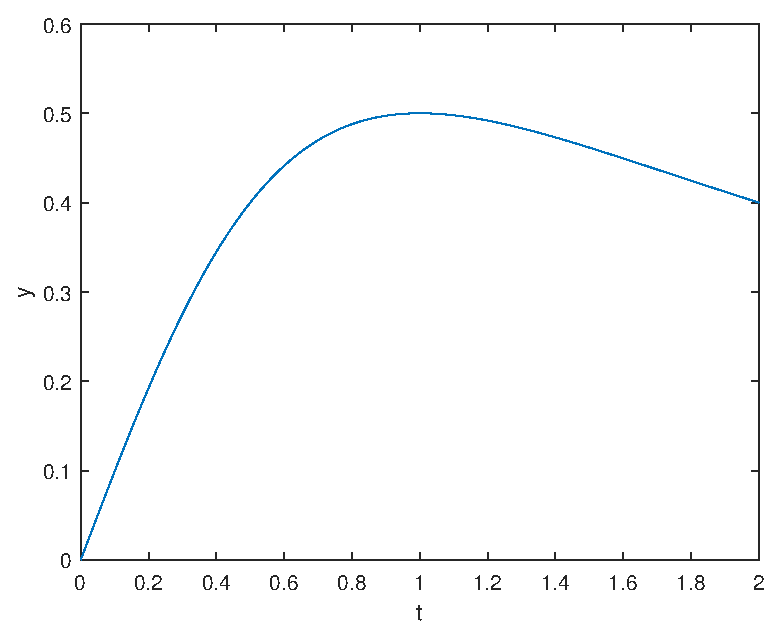
\includegraphics{p2_2_plot.eps}
				\caption{The numerical solution of (\ref{eq:p2_ivp}) on $[0,2]$ with $k = \frac{1}{2048}$ and $\theta = \frac{1}{2}$ -- I promise it's a different figure!}
				\label{fig:p2_part2}
			\end{figure}
			
			\item The table of errors computed by \lstinline{problem2_calculations.m} is given in \lstinline{p2_output.txt} and copied here for convenience (Table \ref{tab:p2:2:b}). It works the same way as in part 1.
			
			\begin{table}[h]
				\centering
				\begin{tabular}{@{}ll@{}}
					\toprule
					$k$ & Error at $t=2$ \\
					\midrule
					1/16 & 4.905053e-05 \\
					1/32 & 1.227079e-05 \\
					1/64 & 3.066097e-06 \\
					1/128 & 7.643168e-07 \\
					1/256 & 1.888337e-07 \\
					1/512 & 4.496056e-08 \\
					\bottomrule
				\end{tabular}
				\caption{Numerical errors at $t=2$ when $\theta = \frac{1}{2}$}
				\label{tab:p2:2:b}
			\end{table}
			
			\item We can estimate the convergence rate of the scheme by using a table. Recall that if $e_1$ and $e_2$ are the errors with $k=k_1$ and $k=k_2$, then, assuming that $\text{error} = Ck^\alpha$, where $\alpha$ is the order, we have
			\begin{equation*}
				\alpha = \frac{\log\left(\frac{e_1}{e_2}\right)}{\log\left(\frac{k_1}{k_2}\right)}.
			\end{equation*}
			Computing the order this way between consecutive errors in Table \ref{tab:p2:2:b}, we see that the order appears to be 2 (see Table \ref{tab:p2:2:c}, which is copied from \lstinline{p2_output.txt}).
			
			\begin{table}[h]
				\centering
				\begin{tabular}{@{}lll@{}}
					\toprule
					$k$ & Error at $t=2$ & Order\\
					\midrule
					1/16 & 4.905053e-05 & -\\
					1/32 & 1.227079e-05 & 1.999041\\
					1/64 & 3.066097e-06 & 2.000752 \\
					1/128 & 7.643168e-07 & 2.004161\\
					1/256 & 1.888337e-07 & 2.017054\\
					1/512 & 4.496056e-08 & 2.070385\\
					\bottomrule
				\end{tabular}
				\caption{Order of numerical errors at $t=2$ when $\theta = \frac{1}{2}$}
				\label{tab:p2:2:c}
			\end{table}
		\end{enumerate}
	\end{enumerate}
\end{document}